\chapter{{Clause, sentence and discourse level phenomena}}

This is the third linguistic chapter with a focus on the salient characteristics of Ship English at the clause, sentence, and \isi{discourse level}. The first section on syntax within the clause presents data on \isi{adverb} use and placement, inherent variation in the prepositional paradigm, intransitive \isi{verb} fronting and the use of both direct and indirect objects. The second section on \isi{subordination} and coordination illustrates the \isi{syntactic complexity} of Ship English with specific attention to strategies of \isi{subordination} and coordination. The last section on swearing as a \isi{discourse marker} explores the role of oath-making and \isi{profanity} in sailors’ speech to mark communicative intent, grammatical modality, individual agency and \isi{group identity}. 

\section{{Syntax within the clause}}%7.1

\subsection{{Adverbs}}%7.1.1

Ship English makes heavy use of prepositional phrases and one clause might feature several adverbial constituents. The two following examples from depositions illustrate heavy use of prepositional phrases with \isi{adverbial function}: “That being at Borligne he was hired by the said Capt Vaughan to serve with him as Master in the barge” [HCA 1/13/95], and “a Prisoner on Board of them Swears, he Several times in that Space addressed to him in French, and with Tears bemoaned his being in Such Company” [HCA 1/99/168]. Many of these prepositional phrases with \isi{adverbial function} occur in the default position of modern standard varieties at the end of the clause, e.g., “and am thies day going with a small vessel for kopon hagen” [HCA 1/101/527] in which the phrases “with a small vessel” and “for kopon hagen” attach to the end of the clause. One word adverbs could also occur at the end of the clause (italicized for emphasis,) e.g., “the tides proved very loe \textit{still}” [ADM 52/2/3], and “they should have Rum \textit{enough}” [HCA 1/99/7]. Adverbial phrases composed of more than one word but not taking a prepositional head also commonly occur at the end of a clause in sailors’ speech, e.g., “several times was threatened \textit{very much}” [HCA 1/99/69] and “John Edwards who came \textit{just then}” [HCA 1/9/51]. However, sailors commonly placed adverbial constituents in a range of positions within the \isi{main clause} whether they were prepositional phrases, single-word adverbs, or adverbial phrases without prepositional heads (see \tabref{tab:key:7.1} and \figref{fig:key:7.1}). 

\begin{figure}
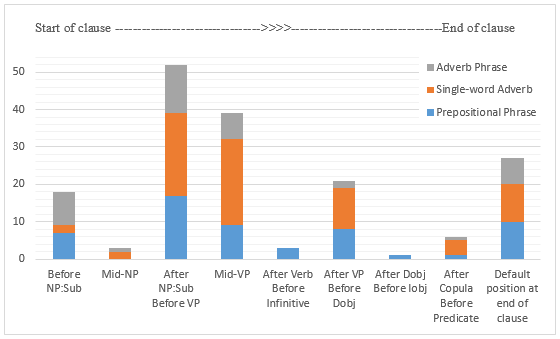
\includegraphics[width=\textwidth]{figures/delgado-img17.png}
\caption{\label{fig:key:7.1} Syntactic placement and type of adverbial constituent in 170 examples.\\
Sources: 1045.f.3, 445f.1, \citet{AdkinsAdkins2008} ADM 106, ADM 51/1, 3954, ADM 52/2, \citet{Brown2011}   CO 5/1411, D/Earle/1/1, DDB6 8/4, HCA 1/9, HCA 1/12, HCA 1/13, HCA 1/14, HCA 1/52, HCA 1/53, HCA 1/98, HCA 1/99, HCA 1/101, Palmer (1986,) SP 42/6, SP 89/34, T/70/1216.}
\end{figure}

  
\begin{figure}  
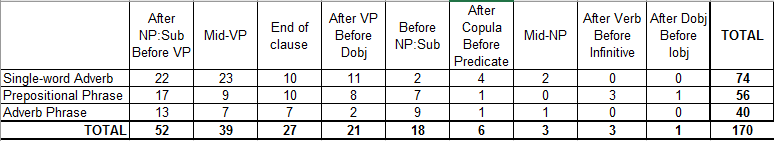
\includegraphics[width=\textwidth]{figures/delgado-img18.png}
 
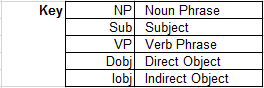
\includegraphics[width=\textwidth]{figures/delgado-img19.png}
\caption{\label{tab:key:7.1} Syntactic placement and type of adverbial constituent in 170 examples, raw data.}
\todo[inline]{figure or table?}
\end{figure}


The most \isi{common placement} for adverbial constituents was after the noun-phrase subject and before the main \isi{verb phrase}. Prepositional phrases (italicized for emphasis) are regularly placed in this position between the subject and main \isi{verb}, e.g., “which they \textit{in a short time} did” [HCA 1/52/88], and “The ship Hastings \textit{in the chase} fired about five \& twenty Gunns” [HCA 1/52/176]. Although the examples given above are short, sailors also inserted long prepositional phrases in this position between the subject and the \isi{verb}, e.g., “The \isi{Mate} \textit{then coming towards him the said John Humphreys} told him that…” [HCA 1/52/124], and “He \textit{with other who had a potentall Comission to take Spanish goods} did seize on them lately at sea” [HCA 1/9/67]. Single-word adverbs and adverbial phrases also commonly occur in this position between subject and the main \isi{verb}, e.g., “hee \textit{well} know” [HCA 1/52/1], “he \textit{lately} belonged to a Spanish frigate” [HCA 1/99/5], “doctors of physic in ships \textit{many times} are very careless” (cited in \citealt{Brown2011}: 47,) and “Manuel Guzman \textit{the second time of Landing} was chosen the officer in Chief” [HCA 1/99 New Providence 1722]. Overall, this post-nominal and pre-verbal position was the most common location for all adverbial constituents in the sample, composing 52 of the 170 examples or 31\% of the total and was the most \isi{common placement} for both adverbial phrases and prepositional phrases with an \isi{adverbial function} (see \tabref{tab:key:7.1}). 

The most \isi{common placement} for single-word adverbs was between an \isi{auxiliary verb} and a verbal \isi{participle}\footnote{\citeauthor{MillwardHayes2012} claim that Early Modern English in general showed a tendency to insert adverbial modifiers between an \isi{auxiliary verb} and a \isi{past participle} (2012: 271-272).}. This occurred with do-support in \isi{indicative modality}, with \isi{perfect aspect}, and with \isi{copula} auxiliaries in both \isi{progressive aspect} and passive constructions, in both indicative and negated statements e.g., “I did \textit{formerly} present to you” [ADM 106/300/21], “The examinant hath not \textit{since} seen him” [HCA 1/14/140], “hee had \textit{long} swam” [HCA 1/53/3], “I am \textit{soone} going to Sea” [HCA 1/101/356], “Which had been \textit{before} taken” [HCA 1/13/95], “Ship that was \textit{lately} cast away” [HCA 1/12/79], and “used to be \textit{often} meditating on the Godly Books” [HCA 1/99/156]. In this position, these single-word adverbs interrupt the verbal phrase, and this effect is more pronounced when the inserted adverbial is either an \isi{adverb} phrase or a \isi{prepositional phrase}, e.g., “Thomas Gardner... did \textit{in June last} take from hence [Deptford] an hoyes Maine saile \& a quantity of Doales” [ADM 106/288/42], “She was \textit{with many of her Slaves} chained” [HCA 1/99/91],  “Juan Boneta Lucrass had \textit{under pretence of that commission} taken Several Sloops” [HCA 1/99/10], and “This informant was \textit{after the sale of the sd ship the Loving Land as aforesaid} put aboard the Gunll of this sd Spanish man of Warr” [HCA 1/53/8]. This interruption is even more pronounced when two or more adverbial interjections are placed in a mid-verbal position, e.g., “Capt Parsons did \textit{in a mornng ab:[about] 9 or ten dayes before Christmas last} call upon this Deponent” [HCA 1/14/54]. In addition to the placement of adverbs between auxiliary verbs and their participles, prepositional adverbs are also permitted to occur after a main \isi{verb} and before an \isi{infinitive} creating a similar effect of interrupting the \isi{verb phrase}, e.g., “he attempted \textit{at Sieraleon} to run away” [HCA 1/99/45], “they were both commanded \textit{in the Boat} to row their Capt on Board”  [HCA 1/99/149], and “you are to be carefull \textit{therefore suly} to observe the sd directions” [CO 5/1411/618]. Although this was not a common feature, it could be seen as an extension of the tendency to place adverbials between auxiliaries and main verbs, which is the most common location for single-word adverbs, and the second most common location for all adverbial constituents in the sample, comprising 39 of the 170 examples or 23\% of the total (see \tabref{tab:key:7.1}).

Further to the most common two placements of adverbial constituents (after the \isi{subject noun} phrase and between auxiliary and main \isi{verb}) Ship English permits other placements with no apparent \isi{linguistic conditioning} by \isi{adverb} type. Adverbial constituents in the sample often occur after the \isi{verb phrase} but before the \isi{direct object} of a \isi{transitive verb}, e.g., “two of them loosing \textit{each} one leg” [HCA 1/12/2], “and has had \textit{since} no opportunities of escaping” [HCA 1/99/125], “the pyrate gave \textit{to the capt} his \isi{longboat}” [CO 5/1411/42], “took away \textit{out of his packett} his Sealed ring” [HCA 1/9/18], and “there was by his order put \textit{into a boate belinging to the St. Andrew} 2 coyles of rope” [HCA 1/101/224]. Similarly, linking verbs permit adverbs before nominal or adverbial predicates, e.g., “become \textit{again} our enemy [445f.1/21], and “he appeared \textit{allways} disconsolate” [HCA 1/99/129]. The \isi{copula} likewise permits adverbs before adverbial predicates, e.g., “Richard Taylor was \textit{a little before} come” [HCA 1/9/39], “He had been \textit{then} dead about foure howers” [HCA 1/9/51], and “Which ship was \textit{abt four years since} run away with” [HCA 1/52/75]. Although the placement of adverbs after verbs and before direct objects or predicates is not common in the sample of 170 sample phrases analyzed, it does suggest that sailors had the option of placing adverbs after verbs regardless of whether the \isi{verb} in question was \isi{transitive}, linking, or \isi{copula} in nature. In short, sailors had the option of locating adverbs in various positions without apparent \isi{linguistic conditioning} by type of \isi{adverbial constituent} or main \isi{verb} type, resulting in patterns of \isi{free variation} in the \isi{corpus}. 

Contrary to this pattern of \isi{free variation}, non-finite adverbial clauses are predominantly located at the start of the matrix clauses in which they occur. Although sailors had the option of placing other types of adverbial constituents (i.e., prepositional phrases, single-word adverbs, and adverbial phrases without prepositional heads) at the start of the clause, fronted adverbial placement was much more common for non-finite adverbial clauses than it was for other types of adverbial constituents. Thus, although phrases with fronted single-word adverbs such as “\textit{likewise} says the captain” [HCA 1/99 New Providence 1722] are evident in the \isi{corpus}, they are not common. Comparatively, sentences with fronted non-finite adverbial clauses occur frequently, e.g., (with non-finite adverbial clauses emphasized in italics) “\textit{upon his threatening to shoot him} he delivered up to him” [HCA 1/99/6], and “\textit{to prevent more of his Impertinence} which she was afraid off went down into the Gun Room” [HCA 1/99/79]. In sum, although we might conclude that single-word adverbs and adverbial phrases have no default placement in Ship English - only a preferred tendency to be placed after the noun-phrase subject and before the main \isi{verb phrase} or in a mid-verbal position between an \isi{auxiliary verb} and a verbal \isi{participle} - when adverbial constituents take the form of non-finite adverbial clauses, they default to a placement at the start of the matrix clauses in which they occur. 

\subsection{{Prepositions} }%7.1.2

Prepositional phrases that are adverbial in meaning are sometimes difficult to identify because Ship English permits the omission of prepositional heads. Prepositional omission occurs with a range of adverbial types, for instance: adverbs of location, “arrived here, [in] his Mars Ship the Tilbury” [SP 42/6]; adverbs of duration, “with Snow [for] most part of the night” [ADM 52/2/3]; adverbs of manner, “wished he had never come [on] the \isi{voyage}” [HCA 1/99/62]; adverbs of comparison, “never having been looked on [as] a Trusty Man among them” [HCA 1/99/151]; adverbs of direction, “then returned him [to] his owne Brigganteine” [HCA 1/98/258]; and adverbs of relation, “he was examined by the Viceadmiral [about] what Companyes of foote were in the Islands” [HCA 1/9/105]. Furthermore, this type of omission which was common to the transcribed depositions and hand-written letters of sailors was also reproduced in print, for instance, the prepositional omission at the head of the \isi{adverb} of manner in a maritime pamphlet “On the 26th past arrived here [on] the Snow Susannah, Capt. Landon from Bristol” [HCA 1/99 The American: Weekly Mercury No.618, Oct 28-Nov 4 1731]. Examples suggest that in such cases the prepositional constituents are indeed present in the underlying structure but perhaps the unstressed nature of the prepositions in speech coupled with high levels of partial literacy among mariners promoted omission in written representations. 

Idiomatic use of prepositions in specific phrases was fluid and highly variable. This is not surprising given that the Early Modern English period was a time in which numerous dialectal differences manifested themselves and there were many new prepositions entering the language owing to the loss of inflection to indicate grammatical relationship (\citealt{MillwardHayes2012}: 268). Limitations of space do not permit a detailed discussion of each \isi{preposition} here, but some examples are illustrated in \tabref{tab:key:7.2} below. 

\begin{table}
\begin{tabularx}{\textwidth}{lQQ}
\lsptoprule
\multicolumn{1}{c}{\textbf{Preposition}} & \textbf{Excerpt} \textbf{Containing} \textbf{Idiom} & \textbf{Source}\\
\multicolumn{1}{c}{At} & Gust at WSW[West South West] & CO 5/1411/706\\
& Piracy at sea is the same with Robbery at land & CO 5/1411/45\\
 & a \isi{longboat} at anchor in Shoar & HCA 1/99/3 Cape Coast {1734}\\
 & he never was at attacking any Ship & HCA 1/99/80 \\
\multicolumn{1}{c}{By} & and by the way mett wth a ketch\footnotemark{} & HCA 1/12/3\\
& missing the Islands by contrary winds & HCA 1/98/267\\
\multicolumn{1}{c}{For} & was for scuttling the Ship & HCA 1/99/22\\
& for till such tyme & ADM 106/288/40\\
 & hee would go for Yarmouth & HCA 1/52/4\\
 & the fleet went for England & ADM 52/1/1\\
 & gave him for answer & SP 89/25/230\\
\multicolumn{1}{c}{In} & evidences in their behalf & HCA 1/99/69\\
& was concerned in taking away the other things & HCA 1/99 New Providence 1722\\
\multicolumn{1}{c}{On} & seize on him & SP 89/25/230\\
& lay hold on the Captain & 445f.1/40\\
 & when on a sudden & HCA 1/99 Barbados {1733}\\
\multicolumn{1}{c}{To} & wee put to sea\footnotemark{} & HCA 1/12/2 \\
& the wind came to no [north] & DDB6 8/4\\
 & there was no violence used to the master & HCA 1/53/67\\
 & aiding \& assisting to all mastors & SP 42/6\\
 & saw a ship to westward & ADM 52/1/1\\
 & in order to your returning to Engld & CO 5/1411/658\\
\lspbottomrule
\end{tabularx}
\caption{\label{tab:key:7.2} Sample of prepositional variation in idiomatic phrases}
\end{table}
\addtocounter{footnote}{-2}
\stepcounter{footnote}\footnotetext{ Although the idiom “by the way” appears similar to the way we might express a parenthetical fact in modern English, the usage in this context means a more literal “on route” (i.e., “on the way.”)}
\stepcounter{footnote}\footnotetext{ This use of the idiom “put to sea” is still used in modern Standard English, sometimes with the \isi{preposition} “out” inserted after the \isi{verb} to create the phrase “put out to sea.”}


Certain combinations with the \isi{preposition} “for” re-occur frequently in the \isi{corpus} but are not necessarily idiomatic. Phrases featuring the combination “for that” can function as complementizers in the same way that the word “that” can when used alone, e.g., “it is untrue, \textit{for that} Scudmore belonged to, and was on Board the \textit{Ranger}” [HCA 1/99/101]. However, other examples suggest that there is a specific meaning attached to the collocation of the two words that act in the same way that the conjunction “because” functions in Modern English, e.g., “he would not do it without the Captains order, \textit{for that} he knew not whether the Captain would allow it” [HCA 1/52/20]. Indeed, this combination appears to mirror the use of the word “for” as a subordinating conjunction when used alone e.g., “[we moored] In 15 fathome, of water \textit{for} it was Calme” [ADM 51/4322/1] and “we kam to Anankor \textit{for} we had the wind att no [north]” [DDB6 8/4]. At other times, the combination of the two words “for” and “that” might have been coincidental, e.g., “if he was \textit{for that} he would defend himselfe” [HCA 1/52/46]. This example can be broken down to mean that the unnamed subject was “for” something, and the something he was “for” is a clause introduced by the subordinator “that,” expressed as “that he would defend himself,” and so the two words “for that,” although they appear to combine in the same way as in the previous examples, are functioning separately. In short, although several examples of the combination “for that” feature in the \isi{corpus}, there is no convincing trend that implies a distinct meaning or an idiom specific to the \isi{speech community} but rather that sailors used the \isi{preposition} “for” as a concordant complementizer or a subordinating conjunction. 

Much more salient than the combination “for that” was the \isi{prepositional phrase} “for to” that occurred specifically by allowing the \isi{preposition} “for” to take an \isi{infinitive} \isi{verb phrase} complement, without an intervening subject, as in present-day Standard English (e.g., “for her to give up now would astound me.” The variety of verbs with which this collocation occurred suggest that the combination of “for to” was not idiomatic but the result of a syntactic rule permitting \isi{infinitive} verbs to follow the \isi{preposition}. Examples of the combination in witness depositions include (with italic and bold emphasis) “it was \textit{for} \textbf{to} \textbf{destroy} what cloathes we had” [SP 42/6], “we were forced \textit{for} \textbf{to} \textbf{lye}” [ADM 52/2/8], and “and \textit{for} \textbf{to} \textbf{satisfie} you” [HCA 1/101/423]. However, the combination was also common in logbooks, e.g., “we waid Anckor and came to sayle \textit{for} \textbf{to} \textbf{make} the best of our way” [T/70/1216/12], “after dinner \textit{for} \textbf{to} \textbf{goo} to the ground” [T/70/1215 Oct 15], and “Recieved Orders from the captain of the \isi{Drake}, \textit{for} \textbf{to} \textbf{Ride} Commandr in Chief” [ADM 51/4322/1]. Miscellaneous letters authored by sailors also show this syntax, e.g., “a Young Man, willing \textit{for} \textbf{to} \textbf{Sacrifice} his life” [HCA 1/101/207], and “All possible Endeavours were rosed \textit{for} \textbf{to} \textbf{heare} her off” [HCA 1/9/155]. Further evidence indicating that the underlying structure of the combination was “for” + [\isi{infinitive}] rather than an \isi{idiomatic usage} of “for to” is that the structure could be interrupted by adverbial constituents, e.g., the word “strictly” in the excerpt “and them \textit{for} strictly \textbf{to} \textbf{examine}” [SP 42/6]. The salience of the “for” + [\isi{infinitive}] structure is highlighted by its representation in several contemporary sea-songs and shanties that were either authored by sailors or written to reflect their speech, e.g., “I met her walking on the Strand / Dressed up \textit{for} \textbf{to} \textbf{beat} the band” \citep[51,]{Hugill1969} “our Lord High Admiral \textit{for} \textbf{to} \textbf{pursue} them sought” (cited in \citealt{Palmer1986}: 8,) “The course / intended \textit{for} \textbf{to} \textbf{Steer}” (cited in \citealt{Palmer1986}: 74,) and “Pork cut in pounds / \textit{For} \textbf{to} \textbf{eat} with our peas” (cited in \citealt{Palmer1986}: 71). The combination “for to” in documents written by sailors, transcribed for sailors, and representing sailors all appear to confirm that the salient use of “for to” occurs because the first \isi{preposition} is permitted to take an \isi{infinitive} complement rather than its occurrence as an idiomatic expression, and this coincides with the usage that \citeauthor{BakerHuber2001} identify as a feature of world-wide English-lexicon contact languages (2001: 201). 

The \isi{preposition} “of” is permitted to combine with other prepositions and often occurs preceding \isi{noun} phrases and pronouns both with and without \isi{genitive} function. Before another \isi{preposition}, examples include “in his Action \textit{of with} the Swallow he Remembers nothing” [HCA 1/99/59], and “and went \textit{of from} the ship” [HCA 1/99/71].  In this latter case, ‘of’ might be an orthographic representation of the \isi{preposition} “off,” which might more commonly combine in such contexts, e.g., “took the Pyrate \textit{off from} beating him” [HCA 1/99/30]. Some of the examples in which the \isi{preposition} “of(f)” follows “out” and refers to a specific location are acceptable in modern \isi{standard usage}, e.g., “they took Capt Macfashion \& Nicholas Simonds \textit{out of} him [the ship]” [HCA 1/99/7] and “mariners sayld \textit{out off} \isi{Jamaica} ten years” [HCA 1/98/7]. Sailors seemingly extended this usage of “of” + [location] to include the \isi{preposition} “aboard,” e.g., “we put men \textit{aboard of} the London” [ADM 52/2/13] and “they could not ship any goods \textit{aboard of} any ship” [HCA 1/99/113 loose letter c. 1730]. When the \isi{preposition} “of” proceeds either \isi{noun} phrases or pronouns, the structure sometimes carries a \isi{genitive}/associative meaning, e.g., “two buineshas [businesses] of him” [SP 42/6], “came down the River of Thames” [ADM 52/1/5], and “the articles of the pyrates” [HCA 1/99/48]. Other examples have a partitive meaning, e.g., “hallf \textit{o(f)} an ouer [half an hour]” [ADM 52/2/1], and “one other \textit{of} the men was order’d to go againe on Board” [HCA 1/99/6]. Yet other uses of the \isi{preposition} appear to have no \isi{genitive} or partitive function, e.g., the excerpt “He would go \textit{of} himself” [HCA 1/9/139] means that he would go “by himself” or alone; “wee were forcd to buy \textit{of} him or goe naked…to buy of him at 10 shillings” [SP 42/6] means “to buy from him;” and “bears witness \textit{of} it” [HCA 1/53/48] means “bear witness to it.” Other examples suggest that “of” could function as a subordinator, e.g., “each time \textit{of} the \isi{prisoner} coming to Cat Island she fled into the bushes” [HCA 1/99 New Providence 1722], or could function as a pseudo-verbal particle after an auxiliary modal, e.g., “they found victualls and sale whar [where] they could \textit{of} it” [HCA 1/53/66]. Although this is a highly marked variant, the use of a \isi{preposition} as a \isi{verb} particle is evident with other prepositions such as the word “up” in the excerpt “we have \textit{up} our anchors” [ADM 52/2/6] and these examples may attest to a feature of sailors’ speech that potentially extended to a number of prepositions. Further examples of the \isi{preposition} “of” seem redundant, e.g., “he should accept \textit{of} it” [HCA 1/99/59], “the Pyrates missing \textit{of} him” [HCA 1/99/64], and “the Duch squadrn that Came in yesterday counting \textit{of} about 12 Saile of men of war” [ADM 52/2/5]. Although such examples were few, and there is no significant trend showing non-standard sage of the \isi{preposition} “of” in Ship English, these excerpts attest to a variation that extended well beyond \isi{genitive} and partitive functions familiar to modern \isi{standard usage}. 

\subsection{{Variation in SVO order: Verb fronting}}%7.1.3

Ship English permits intransitive verbs to be expressed before noun-phrase subjects in simple clauses. This structure occurs with independent verbs, with phrasal verbs, and with \isi{verb} phrases which include auxiliary constituents. Intransitive verbs used independently (i.e., as the sole constituent of the \isi{verb phrase}) often precede their \isi{noun phrase} subjects, e.g., (with verbs italicized and \isi{noun} phrases in bold for emphasis) “\textit{began} \textbf{a} \textbf{very} \textbf{Sore} \textbf{Storme} \textbf{of} \textbf{Wind}” [ADM 52/2/3], “if \textit{blows} \textbf{any} \textbf{wind}” [CO 5/1411/640], “\textit{appeared} personally \textbf{Thomas} \textbf{Colston}” [HCA 1/14/17], “\textit{Stayed} for the stern \textbf{most} \textbf{ships} all night” [ADM 51/3954], and “still \textit{continued} \textbf{much} \textbf{wind}” [ADM 52/2/5]. When intransitive verbs incorporate a \isi{satellite particle} they are also permitted to precede their \isi{noun phrase} subjects, and this is most notable with the \isi{verb} “to come,” e.g., “\textit{came in}: \textbf{2} \textbf{Jamaica} \textbf{Sloops} from \isi{Barbados}” [ADM 52/1/7], “Yesterday in the afternoon \textit{came hither} \textbf{Captn} \textbf{Wm} [William] Passenger” [CO 5/1411/659], and “Last night \textit{came aboard} \textbf{5:} \textbf{hhs} \textbf{[hogsheads]} \textbf{of} \textbf{beefe}” [ADM 52/1/8]. Indeed, fronted \isi{verb} phrases using “to come” appear to have been a salient marker of sailors’ speech and are recorded in sea-songs of the \isi{seventeenth century} such as “A Joyful New Ballad” that includes the line “First \textit{came up} \textbf{their} \textbf{admiral}” (cited in \citealt{Palmer1986}: 25). Verb phrases which include auxiliary constituents also precede their \isi{noun phrase} subjects, e.g., “\textit{was coming} \textbf{a} \textbf{soldier} to Cape Coast Castle” [HCA 1/99/28] and “The day following \textit{were landed} \textbf{7000} \textbf{foot} \textbf{soldiers}” [BL/Egerton 2395/0003]. This common feature of verbs proceeding their \isi{subject noun} phrases appears to be conditioned by the intransitive nature of the \isi{verb} itself and is unaffected by the composition of the \isi{verb phrase} as either an independent \isi{lexeme}, a \isi{phrasal verb} with \isi{satellite particle}(s,) or a complex \isi{verb phrase} with auxiliary constituents. 

Many of the examples cited in the paragraph above attest to the commonality of adverbial constituents preceding fronted intransitive verbs. Repeated use of adverbs was evident throughout the \isi{corpus} and may reflect the informative purpose of many of the documents studied, yet it may have also provided the \isi{linguistic conditioning} that enabled intransitive verbs to assume a position prior to the \isi{noun phrase} subject. Although some of the adverbial constituents involved do not relate to time, e.g., (italicized for emphasis) “\textit{likewise} says the captain” [HCA 1/99 New Providence 1722], most examples in the \isi{corpus} where an \isi{adverbial constituent} precedes a fronted intransitive verbs are adverbs of time, such as the excepts from the following depositions: “\textit{In the after noon} came in the Tiger Prize” [ADM 52/1/7], “\textit{at seaven in the morning} came in a fine ship” [ADM 52/2/3], and “\textit{Towards the evening} came both on board” [HCA 1/9/3]. Logbooks also show this syntax, e.g., “\textit{In the morninge} Came a little wind” [ADM 51/4322/1], “\textit{This morninge} Came one Board of us: some cannewse[canoes]” [T/70/1213], and “\textit{In the morning} died one of our sea men and \textit{in the After noon that day} died our dorktor” [T/70/1213]. Likewise, journals show the presence of adverbial constituents preceding fronted intransitive verbs, e.g., “\textit{Within few days after} followed the generals” [BL/Egerton 2395/0003], and “\textit{Then} said I to the Men” [445f.1/36]. Thus, the placement of intransitive verbs before their \isi{noun phrase} subjects was a wide-ranging feature in the \isi{corpus} that was potentially motivated by constructions where adverbial constituents relating to time preceded fronted verbs.  

The placement of verbs before the subject is predominantly associated with intransitive verbs, yet there is limited evidence of this syntax also occurring with linking verbs, \isi{transitive} verbs, and as part of pseudo-\isi{expletive} structures. The example “then began I to think” [445f.1/35] shows how this occurs with a \isi{linking verb}, and “often being all Hands Drunk” [HCA 1/99/91] shows its occurrence with the \isi{copula}. The examples “don’t you see says he them two ships” [HCA 1/99/105] and “the following bills delivered the attorney General” [HCA 49/98/106] also illustrate how verb-subject inversion may occur with a \isi{transitive verb}, and this even extends to passive constructions, e.g., “today [was] Taken out of the George Hoy Tho Harris, Mr.” [ADM 52/1/5]. Expletive structures composing the word “there” and the \isi{copula} before a \isi{predicate noun} phrase functioning as the \isi{logical subject} technically do not permit the \isi{verb} before the subject which is grammatically represented by the word “there,” (in italics for emphasis) e.g., “\textit{there}\textbf{ }are the principal ports on each side” [1045.f.3/1/16]. However, variations of this structure in which the word “there” does not function as a \isi{grammatical subject}, in which it is replaced by an adverbial locative “there” appear to feature verbs occurring before their \isi{noun phrase} subjects. The examples “\textit{there} hapned a very great storme” [HCA 1/14/16] and “\textit{there} appearing several persons” [HCA 1/99/50] appear to use the word “there” as a \isi{grammatical subject}, yet the verbs “to appear” and “to happen” are not typical in \isi{expletive} constructions and so cause the word “there” to be interpreted as an \isi{adverb} rather than a \isi{grammatical subject} and this consequently means that the only logical \isi{noun phrase} subject occurs in a position after the \isi{verb}.  The same kind of effect occurs in the example “for \textit{here} commonly runs a great Sea” [1045.f.3/1/26] in which the word “here” suggests a \isi{logical subject} in the same way that “there” does in existential structures, but is interpreted as an \isi{adverb} meaning “here in this place” rather than a pronominal constituent and so the only \isi{noun phrase} in the clause, “a great sea,” occurs after the \isi{verb} “to run.” Even followed by the \isi{copula}, the word “here” can be interpreted as an \isi{adverb} rather than a \isi{grammatical subject}, e.g., “They build with Fig-Tree[s]; \textit{here} being, as I was told, no other Trees fit to build with” [1045.f.3/1/27]. The limited number of examples that show a fronted \isi{verb} that is either linking, \isi{transitive}, or used as part of a pseudo-\isi{expletive} construction may indicate that some sailors extended the scope of intransitive \isi{verb} fronting, however, given the small number of examples available, it may also show idiolectal variation within the \isi{speech community}.  Research on this specific feature with a larger sample might show that conditioned variations were permitted with verbs that were not intransitive; it might also indicate potential \isi{language change} within the community as the feature of \isi{verb} fronting began to widen in its linguistic scope beyond its common intransitive context. 

\subsection{{Direct and indirect objects} }%7.1.4

Evidence from sailors’ speech and contemporary sea-songs of the late sixteenth and early seventeenth centuries suggest that direct objects may have been moved to an initial position, i.e. OSV word order. Sailors sometimes expressed direct objects at the start of the clause in which they occur, e.g., (italicized for emphasis) “\textit{this fellow} I did not see” [CO 5/1411/36] and “\textit{this} we will do” [445f.1/37] in addition to the standard expression of the \isi{direct object} after the subject and main \isi{verb}, e.g., “we culd see \textit{her} no longer” [DDB6 8/4]. The fronting of direct objects among sailors may have been a salient feature of their speech given that it occurs in contemporary sea-songs and shanties several times, for example, it occurs twice in the late sixteenth-century song “Lustily Lustily” in the lines, “\textit{Nothing} we want” and “\textit{ourselves} we will try”\footnote{This excerpt is taken from the line “Like worthy mariners \textit{ourselves} we will try” in which the reflexive “ourselves” functions as the \isi{direct object} of the \isi{transitive verb} “try” and thus creates the meaning “we will try ourselves” (i.e., put our own actions on trial). Although out of context, the reflexive may appear to function as an \isi{emphatic} marker (i.e., we \textit{ourselves} will try [to do something]) the absence of an \isi{infinitive} complement in the clause or an associated \isi{verb phrase} in the adjacent lines of verse weakens the validity of such an interpretation.}  (both cited in \citealt{Palmer1986}: 2) and it occurs twice in the early seventeenth-century song “Another of Seafarers....” in the lines,  “\textit{A happy end} I do require” and “\textit{Gentle calm} the coast will clear” (both cited in \citealt{Palmer1986}: 6). Sea-songs of the period also suggest that sailors were known to place \isi{predicate noun} phrases at the front of a clause after the \isi{copula} in the same manner as a \isi{direct object} might undergo fronting, e.g., “\textit{My eldest daughter} thy wife shall be” (cited in \citealt{Palmer1986}: 48,) yet there is no evidence in the \isi{corpus} of sailors’ speech that attests to this potential extension. Thus, although the evidence from the \isi{corpus} of Ship English does not suggest the same level of salience that the contemporary sea-songs suggest, evidence shows that sailors did sometimes locate direct objects at the start of the clause. 

Direct objects might be expressed after a \isi{nominal subject} and before the main \isi{verb} in a clause. Sea-songs suggest that sailors might have expressed the \isi{direct object} of \isi{transitive} verbs after a \isi{pronoun} (in bold for emphasis,) e.g., “Let \textbf{him} \textit{his native soil} eschew” and “To haughty hearts \textbf{who} \textit{fortune} seek” (both from the song “In Praise of Seafaring Men, cited in \citealt{Palmer1986}: 4). In addition, one example of a predicate \isi{adjective} (italicized) located after a \isi{noun phrase} and before the \isi{copula} suggests a similar structure: “\textbf{our} \textbf{prayers} \textit{so fervent} were” (from the song “Sailors for my Money” cited in \citealt{Palmer1986}: 45). Although there was no evidence in the \isi{corpus} of sailors’ speech that attests to direct objects occurring between subject pronouns and \isi{verb} phrases, some examples in which the subject is omitted shows the \isi{direct object} occurring before the \isi{verb phrase} suggesting similar underlying syntax, e.g., “send for the severall men brought in by Captain Legg, and \textit{them} \textbf{strictly} \textbf{to} \textbf{examine} \textbf{apart}, and of them enquire whither the said sloop was bound” [SP 42/6/52]. The excerpt in bold “them strictly to examine apart” is interpreted as a clause meaning “you will examine them separately and strictly” and as such, the absence of the \isi{subject noun} phrase and \isi{auxiliary verb} is explained by the \isi{imperative modality}. However, the \isi{verb} “examine” in standard syntax should precede both the \isi{direct object} and any \isi{adverbial constituent} (in that sequence,) yet the excerpt “them strictly to examine” expresses the \isi{direct object} “them” first, followed by the \isi{adverb} “strictly” and then the \isi{verb} “examine” showing variant placement of the \isi{direct object} in the underlying syntax regardless of where the \isi{noun phrase} subject might have been placed. Further support for this interpretation is suggested by a maritime pamphlet that features two statements in which the subject is omitted (here shown in parenthesis) and the \isi{direct object} of the \isi{verb} (in italics) precedes the \isi{verb}: “and then and there \textit{the said ship and her Cargoe} [they] did Piratically and feloniously steal take and carry away” and “\textit{the said Ship} [they] did Piratically and Feloniously sink and destroy” [both from HCA 1/99 The American: Weekly Mercury No.617, Oct 21-Oct 28 1731]. Thus, although supporting evidence is limited, it is possible that variant placement of the \isi{direct object} after the subject and before the main \isi{verb} in a clause was permitted, even when the subject was expressed in \isi{pronominal form} or was not realized in the surface structure. 

Limited evidence suggests that direct objects may have been omitted from clauses featuring \isi{transitive} verbs. The most common occurrence of \isi{direct object} omission took place in logbooks, and specifically in contexts where the \isi{direct object} of the \isi{verb} is self-evident, e.g., “This Day att 10 in the Mouning wee weayed [anchor]” [DDB6 8/4]. Of course, it is possible that the \isi{verb} “to weigh” is being used as an intransitive \isi{verb} in such contexts, yet the more common usage of the word (even in nautical contexts) as a \isi{transitive verb} that occurs explicitly with the \isi{direct object} “anchor” diminishes the likelihood of intransitive use. Further to the specific example of “to weigh” in logbooks, personal communications and witness depositions also suggest that direct objects could be omitted with other normally \isi{transitive} verbs. For example, Captain William Hennesey’s letter to an Admiralty official regarding a quantity of money that he has yet to receive explains that he is writing “although demanded [the money] of him before” [ADM 106/300/35]\footnote{Although the context of the letter makes it clear that the author is referring to payment, there is no explicit reference to a \isi{direct object} (e.g., “money” or “wages”) in the clause that might serve as an antecedent referent.}  the deposition in which the witness explains how pay was promised to the \isi{crew} but never materialized, even after a promise the captain made “to give the men [extra pay] for extraordinary works” [SP 42/6]. Depositions omit direct objects when they may have been realized as pronouns, e.g., “I made [him] lye downe his swoard” [SP 42/6] and “his owne safety \& conscience obliged [him] to it after” [SP 42/6 17 Aug {1700}]. Interestingly, the second example includes the \isi{direct object} “him” (here shown in parenthesis) written in the margin of the transcribed testimony, presumably added as a correction after the initial testimony was transcribed. Hence, the initial transcription without an explicit \isi{direct object} might have been more closely reflective of the speech of Henry Atkinson who was making the testimony and potentially more reflective of common speech of sailors rather than the Standard English that court clerks would have been expected to use. In short, such evidence might suggest that sailors not only permitted the fronting of direct objects but may also have omitted them from speech altogether in contexts where the object referent was understood from context.  

Indirect objects expressed after the \isi{direct object} are often used without either the \isi{preposition} “to” or “for,” contrary to standard \isi{modern usage} that requires a \isi{prepositional phrase} in contexts where indirect objects follow the \isi{direct object}.\footnote{\citeauthor{MillwardHayes2012} explain that Middle English saw an increase in the use of prepositions to clarify the relationships between constituents of a sentence that no longer carried the distinctive inflections of Old English determining grammatical function. (2012: 178). Regarding the use of prepositional particles with indirect objects, they explain that since Old English, when both indirect and direct objects are present in a clause in the DO+IO order, the construction may occur without a prepositional particle, e.g., Shakespeare’s “’twas men I lack’d, and you will give \textit{them me}” (Henry VI, Part 2,c. 1591, 3.1.345). They further stress, “this option is still available in British English, but has been lost in American English, where give me it is acceptable, but give it me is not.” (\citealt{MillwardHayes2012}: 321).} Sailors sometimes expressed indirect objects (italicized) after prepositions (in bold,) e.g., “to make room \textbf{for} \textit{him}” [SP 42/6] and “to fetch provisions \textbf{to} \textit{the others}” [HCA 1/99 New Providence 1722]. Yet more commonly, when the indirect object occurs at the end of the clause, it is used without a \isi{preposition}. The archetypical \isi{verb} that demands a \isi{direct object} and an indirect object, “to give,” shows this prepositional omission most clearly, e.g., “liberty was given \textit{me} to go” [CO 5/1411/28], “Orders will be given \textit{you}” [CO 5/1411/658], “he did not give it \textit{him}” [SP 42/6], and “They had Brandy given \textit{them}” [HCA 1/9/14]. Other verbs that necessitate both direct and indirect objects are expressed with comparable syntax, e.g., “which was granted \textit{me}” [1045.f.3/1/10], “I shall lose all my mony \textit{him}” [HCA 1/101/317], “he brought his privities \& showed them \textit{me}” [HCA 1/99/4], and “we had a pilot ordered \textit{us}” [ADM 52/2/9]. It is possible that sailors did not assign a great deal of importance to expressing indirect objects, as exemplified by two court depositions in which they are added in superscript by the \isi{court clerk}, “his unjust dealings \textsuperscript{to us} may meet him” [SP 42/6], and “made him lay down his swoard, but gave it \textsuperscript{him} again” [SP 42/6]. However, even when expressed, indirect objects were not required to follow prepositions when placed after the \isi{direct object}, as in modern \isi{standard usage}, e.g., “give \textbf{it} \textit{to me}” but were permitted to stand alone as complementary object constituents to the \isi{transitive verb}. 

\section{{Subordination and coordination}}%7.2

\subsection{{Syntactic complexity}}%7.2.1

The \isi{corpus} of written Ship English is notable for its complexity in terms of clause \isi{subordination} and extensive use of adverbial phrases\footnote{I acknowledge that various documents in the \isi{corpus} were extremely difficult to evaluate at the syntactic level owing to the frequent instances of incomplete or damaged documents and illegible text because of handwriting style, unfamiliar symbols, and ink stains, fading and discoloration. Syntactic analysis was also impeded by unconventional \isi{punctuation} and capitalization that does not always make it clear where sentence breaks were intended. Thus, the \isi{corpus} of material from which I could draw data for this analysis was significantly reduced in comparison to the data available for analysis of \isi{noun} and \isi{verb} phrases in Chapters 6 and 7.} . It may be that such complexity derives, at least in part, from the stylistics expected from formal letter writing during the period. One letter (reproduced in full below) dated 1700 and addressed to the Admiralty is punctuated as a single sentence: 

\begin{quotation}
My lords of the Admiralty - having received an acct from Capt Fairbourne, who Commands the ships last sent to Newfoundland, that he has suspended Lieutenent Lilburn the chief officer of the Forces at Newfoundland, I am Commanded by their Lordsps to send you the Copy of Capt Fairbourne’s letter, as also of the severall affidavits and Complaints which ledd him to the doing thereof, and am to desire that you will lay the same before the Rt honble Mr Secretary Vernon I am your most humble servant. [SP 42/6/3] 
\end{quotation}

The \isi{primary clause} of the letter is expressed in the passive voice: “I am Commanded by their Lordsps to send you the Copy of Capt Fairbourne’s letter” and starts after 35 words (nearly 40\% of the 88-word letter) which together comprise a \isi{noun phrase} salutation, an \isi{adverbial phrase} providing sequential information, two relative clauses (one embedded within the other,) and a \isi{noun phrase} appositive giving additional information about the \isi{direct object} of the second embedded \isi{relative clause}. After this \isi{main clause}, there is another \isi{adverbial phrase} of association with an embedded \isi{relative clause} and a further subordinate clause that is coordinated by the conjunction “and” but lacks an explicit \isi{nominal subject} (assumed to be the same first person as the \isi{primary clause}) and a conclusive \isi{prepositional phrase} that is adverbial in function. All of this runs onto an unpunctuated but independent clause that concludes the letter with a customary salutation. Frequent \isi{subordination} and insertion of adverbial information in letters such as these created extraordinarily complex sentences and seem to suggest that mariners favored \isi{syntactic complexity} in letter-writing.  

To contextualize this epistolary \isi{syntactic complexity}, we must remember that short but syntactically-complex letters were commonplace during the period when letter-writing was encouraged as “a practical skill for the rising classes” \citep[178,]{Mitchell2007} yet was promoted through letter-writing manuals and explicit instruction in vocational schools that emulated Latin models (see Webster \citeauthor{WebsterNewbold2007}’s “Letter Writing and Vernacular Literacy in Sixteenth-Century England” 2007: 127-140). Classical models promoted multiple complex structures with rhetorical devices and biblical and metaphorical allusions that were explicitly composed to demonstrate learning and status. \citet{MillwardHayes2012} further explain that promotion of Classical syntax was on the rise in the Early Modern English period due to the revival of Classical learning throughout the Renaissance, and thus:

\begin{quotation}
“Elegant” English came to be characterized by long, heavily subordinated, periodic sentences (as in the opening lines of The Canterbury Tales) and by such devices as parallelism, couplets, balanced clauses, and use of absolute participles (as in “Today being the 4th of July….”) At the same time, the older, native tradition of cumulative, paratactic sentences was never completely lost. (\citealt{MillwardHayes2012}: 275).
\end{quotation}

The result was that generations of aspiring midshipmen, who were often relied upon to compose routine communications, wrote in ways that emulated a heightened Latinate style. Higher-ranking officers composing their routine communications in English would also have defaulted to stylistic devices learned as part of their education in the prestigious Latin models. It would appear that, as a result, heavily subordinated syntax is favored even in communications of a basic nature. To illustrate, one senior officer writing a letter to inform a colleague of his arrival in New York composes a complex series of subordinating clauses and adverbial constituents before coming to the point after nearly 70 words of his opening sentence.

\begin{quotation}
Tho I had great cuase to have expected your Return to Boston at the time of my arrival to this place, one of my Governments [government men] which his Majesty has been pleased to committ to my Charge, but being Informed by the ships that Lately came from Madagascar that you were upon a further cruse, and did not doubt of your makeing of a good voyadge, I have therefore thought fitt by this opportunity to acquaint you of my arrivall… [HCA 1/98/128.]
\end{quotation}

Thus, even when the intentions of the authors were to communicate relatively simple messages, their letters are often composed with a heightened style incorporating heavy \isi{subordination} and complex syntax more suited to classical rhetoric. However, as this was a trend among literate classes during the period, although it features in the \isi{corpus} of Ship English, it is not necessarily a trait that sailors expressed more than any other literate population of the time. 

Sailors’ depositions also incorporate significant complexity within clause structure and this may be explained by considering that the formality of the context that promoted complexity and \isi{subordination} in sailors’ letters may also have influenced their formal speech.  One excerpt from a transcribed witness statement, dated March 28 1722, narrates the events of a \isi{pirate} attack:

\begin{quotation}
About Eleven a Clock, She being come within Pistol Shot A Brest of Us, and a black Flag, or Pendant, hoisted at their main Top Mast Head, We Struck the French Ensign, that had continued hoisted at our Staff till now, and displayed the Kings Colours, giveing her at the Same time our Borad side, which was immediately returned by them again but with unequal Damage, their Mizon top Mast falling, and some of their rigging being disabled… [HCA 1/99/14] 
\end{quotation}

The \isi{primary clause} “We Struck the French Ensign… and displayed the Kings Colours” is proceeded by a \isi{prepositional phrase} functioning as an \isi{adverb} of time, a \isi{participle phrase} functioning as a pseudo-subordinate clause (see Chapter 5 §Present Participle Phrases) and an \isi{adverbial phrase} linked by the conjunction “and” but missing a prepositional head. Following the \isi{main clause} (which is itself interrupted by a \isi{relative clause}) comes another \isi{participle phrase} with an embedded \isi{relative clause} and an \isi{adverbial phrase} linked by the conjunction “but.” The utterance concludes with an absolute phrase (a clause missing its auxiliary) and another \isi{participle phrase} with pseudo-subordinate clause status. Frequent \isi{subordination} and insertion of adverbial information in transcribed depositions such as these suggests that mariners favored \isi{syntactic complexity} in speech as well as in letter-writing\footnote{The caveat remains however that the \isi{syntactic complexity} may be owing to the \isi{court clerk}’s composition, \isi{punctuation}, and style of reporting the speech rather than an accurate representation of the spoken mode.} . 

It may be argued that emotive depositions such as the one cited above in which the speaker reflects on the events of a \isi{pirate} attack are more prone to complexity in expression as the speaker unconsciously reflects the confusion and pace associated with the event in their syntax. However, excerpts from witness testimonies that relate commonplace events with presumably little emotional agitation also feature complex syntax. For example, one witness explanation of how a defendant entered service on a specific vessel along with some other sailors features syntax comparable to the previous narration of a \isi{pirate} attack:

\begin{quotation}
He being a foremast man of his Ma[jes]ties Ship the Phenix Capt John Ferrell Comander upon takeing of a ship called the \textit{Blessing} in Paratt Roade was together with Lieutenant William Bing (who was made Comander of her) James Green James Lynam Richard Cravat James Harrison Robert Day and severall others put on board of the said ship \textit{Blessing} by the order of the said Capt Ferrell, to serve in her. [HCA 1/52/127]
\end{quotation}

The \isi{primary clause} of this utterance “He…was… put on board of the said ship \textit{Blessing}” is interrupted by various adverbial constituents and relative clauses that provide circumstantial information and significantly obscure the clarity of the \isi{main clause}. Although it is not assumed that this memory prompts any emotive agitation from the witness making the statement, it reflects \isi{syntactic complexity} with multiple \isi{subordination} nonetheless and suggests that this manner of speech may have been customary among sailors in the formal context of the court. 

Although the formality of writing letters or making \isi{court testimony} may have prompted a degree of \isi{syntactic complexity}, the complexity observed in the \isi{corpus} of Ship English under study certainly may reflect the spoken mode itself\footnote{As discussed in \sectref{sec:1.3.2}, over half of the materials in the \isi{corpus} derive from court records which feature testimony composed in spoken mode and transcribed. Thus, although I consider the excerpts of such testimony as representative of the spoken mode I acknowledge that they are written documents and potentially ambiguous sources with which to discuss syntactic features representative of spoken modality.} . Speech acts need not adhere to the rules that restrict clause composition in writing conventions and are not defined by \isi{punctuation} or paragraphing. Speech is also a mode in which prosody, pitch, and normative expectations shared by the speaker and hearer shape meaning in such a way that its representation in prose (particularly without \isi{punctuation}) is difficult to follow, for instance one witness’s response when asked if a \isi{prisoner} had any share of stolen goods reads, “yes he had all the pyrates had shared they were all sent for to go upon the quarter deck” [CO 5/1411/78]. Another witness testimony is difficult to follow in prose owing to the extent of adverbial interjections that may have been spoken in a different tone to aid clarity in oral communication:

\begin{quotation}
Harry Glasby that at first the Man was forced for he Saw the Quarter Master Goe who had told he wou’d being all the Enef Men out of this Dutch Interloping Ships that he belong’d to but that he had Opportunity enough as had all of them to have left the Pyrate Ship at Sieraleon if the pleased [HCA 1/99/105.]
\end{quotation}

Some transcriptions include transitional markers to aid reader comprehension, such as the words “first” and “second” in the following example, yet remain challenging to decode at first sight without the aid of conventional \isi{punctuation}: 

\begin{quotation}
they mett wth unother Dutch man with 12 Guns and 32 or 33 men the first yeilded without fighting the second did fight agood while and at last yeilded he gave them quarter he had 4 or 500 small barrells of brandy on board he took their best Guns and so let them go [CO 5/1411/98.]
\end{quotation}

\citeauthor{Givón2001} explains that speech does not reflect the traditional dichotomy between declarative and non-declarative clauses that writing distinguishes, instead it is a much more fluid mode that features clusters of categorical peaks which communicate meaning along a multi-dimensional continuum (2001: 288). Hence, the complexity of the syntax in witness depositions may derive from the rapid syntactic and categorical shifts that commonly occur in spoken forms. Indeed, when authors of narrative fiction attempt to reflect free-indirect speech, they consciously increase the frequency of subordinating particles, embedding and disruption of the finite clause with coordinated non-finite clauses and incongruent phrases juxtaposed by coordinating conjunctions (\citealt{Sotirova2016}: 181). So, although written representations of speech in the form of letters and transcribed testimony may have prompted their own \isi{syntactic complexity} owing to the conventions of the context, the modality of speech itself is inherently complex and likely to include multiple adverbial phrases and subordinating clauses that may or may not be coherent when disassociated from the deixis of their original spoken form.   

\subsection{{Subordinators}}%7.2.2

Given the \isi{syntactic complexity} of Ship English illustrated above, subordinators feature heavily in the \isi{corpus} to organize and embed linguistic units in larger structural hierarchies. One salient marker of \isi{subordination} (discussed in Chapter 5) is the use of \isi{present participle} phrases that function at the clause level by providing attendant circumstances, e.g., (with the subordinated clause italicized for emphasis) “Shipp Albermarle Undocked \& Took in 70 Tunn of Ballast \textit{we having 30 Tun of Ballast Remaining in the Shipp}” [ADM 52/2/5] and “I likewise advised him how dangerous it was to have in such amount Villains Aboard \textit{they having the command of his small Arms}” [HCA 1/98/271]. These subordinate structures commonly take the \isi{participle} form of the \isi{copula} and function in a manner equivalent to using the inflected form of the \isi{verb}, e.g., “Lancaster Sayled hence for Portsm \textit{she being very Leakey}” [ADM 52/2/5] and “Their shipp on fire \textit{she being so Disabled}” [ADM 52/3/7]. See 5. Noun Phrases, and §Present \isi{participle} phrases and §Phrases headed with “being” for full discussion.

The \isi{lexeme} “that” features heavily in the \isi{corpus} as a subordinator of dependent clauses in addition to its function as a \isi{relative pronoun}. The following example demonstrates the use of both functions (subordinator in italics and \isi{relative pronoun} in bold):

James Munjoy Cooper of the same Ship - Deposed \textit{that} he saw Smith beat and forced into the Boat from them, \textit{that} when he returned again with Leave of the Pyrates for Some things of his own \textbf{that} were left, they would not trust him [HCA 1/99/21.]

The first use of the \isi{lexeme} “that” in the excerpt “Deposed \textit{that} he saw Smith…” functions as we might anticipate its use in Modern English, to mark a clause that is subordinated into the role of a \isi{noun phrase}, specifically the dependent clause functions as the \isi{direct object} of the \isi{verb} “deposed.” Interestingly, this type of \isi{standard usage} is often associated with phrases that appear to feature the voice of the \isi{court clerk} or official rather than the deposed \isi{sailor} himself, e.g., “this Deponent further saith, \textit{that} in Corasao” [HCA 1/53/67], “The Prisoner owned his being on board, and the Robbery but \textit{that} any Irregularities he might commit, was the Drink” [HCA 1/99/40], and “he knew no more of the matter, [other] than \textit{that} they were all very drunk” [HCA 1/99 Cape Coast of Africa, Feb 4 1734, 5]. It may be that this type of \isi{standard usage} owes more to the compositions of the clerks transcribing the depositions or the literate court officials surmising court proceedings than the syntactic choices of the speakers themselves. Furthermore, this interpretation of \isi{standard usage} associated with educated clerks can be supported by its occurrence in formal letters written by literate sailors, e.g., “I...am to devise \textit{that} you will lay the same before the rt. hon. Mr. Secretary Vernon” [SP 42/6] and “I hoped ere this to have finisht the repaire of the Hulle but this bad weather hath prevented, \textit{thatt} yett wee want three or fower faire dayes" [ADM 106/288/15]. Thus, although the standard use of “that” as a subordinator for dependent clauses in larger matrix clauses exists in the \isi{corpus}, it may reflect the compositions of literate sailors and court officials rather than usage among illiterate \isi{crew} who were not formally educated. 

If one function of the \isi{lexeme} “that” was to mark literacy and formality (and therefore also status) it is not surprising that sailors who were not formally educated appropriated the word to increase their perceived status in the court and lend credibility to their testimony.\footnote{Although here I discuss the use of the word “that” in court depositions as they show the most frequent occurrence of the phenomenon, it is also evident in logbooks, e.g., “Very Hard Gales - \textit{that} we was forsed to Stand to the Westward” [ADM 52/1/1]. It also occurs in official communications with the Admiralty, e.g., “My lords of the admiralty, having received an acct. from Capt. Fairbourne who commands the Ships last sent to Newfoundland, \textit{that} he has suspended Lieutenant Lilburn the chief officer” [SP 42/6.]}   The \isi{lexeme} “that” is repeated numerous times in \isi{court testimony} in ways that do not correspond to its function either as a \isi{relative pronoun} or as a subordinator, and this may reflect the hypercorrection of uneducated sailors. The most common variant usage of “that” in sailors’ testimonies was to mark the opening of an independent clause, e.g., “\textit{That} Roberts the Commander of the Pyrate Ship, also himself told him the said Smith was and shou’d be compelled into their Comapny” [HCA 1/99/21], “Sammuel Sterling knows him, \textit{that} his Friends were well to pass” [HCA 1/99/92], “if some design he was about proved successfull, \textit{that} he should no longer have occasion to use the sea” [SP 42/6], and “he was kept aboard the Pyrate, \textit{That} this \isi{prisoner} had a pair of Buckles” [HCA 1/99 \isi{Jamaica} Aug 11 1740]. The logical connection between some of the clauses connected with “that” may suggest that sailors were using “that” as a coordinating conjunction. However, examples of the word in juxtaposition with coordinating conjunctions appears to discredit this interpretation as they would render the word “that” redundant as a conjunction, e.g., (with both words marked for emphasis) “The Carpenter had been beaten by the Mr Wm Parsons \textit{and that} he dyed shortly after” [HCA 1/52/176] and “the Prisoner should not go, \textit{for that} he wanted a Polite…[indecipherable]” [HCA 1/99 \isi{Jamaica} Aug 11 1740]. The word “that” is also often juxtaposed with subordinating conjunctions that similarly render the word “that” redundant as a subordinator e.g., “some time \textit{after that} I write you last” [HCA 1/99 loose letter c. 1730], “but know no Particulars \textit{unless that} he wou’d often be merry and Drinking as others” [HCA 1/99/120], “Here is A great depression of her \textit{BeCause that} She layeth Here with A faire wainde [wind]” [HCA 1/101/555], and “\textit{That when} the murderers were asleep they fell upon them” [both from HCA 1/99/10]. In short, it is possible that the context of complex language and expectations of formality in the courts of the Admiralty and official communications with them conditioned the use of “that” as a \isi{discourse marker} to index status and this explains why so many samples contain independent clauses that feature the word in a manner that has no apparent \isi{syntactic function}.

In contrast to the suggestion that the \isi{lexeme} “that” was appropriated by uneducated sailors and inserted erroneously in speech, there is evidence that it was used to form cumulative super-structures that may have been punctuated incorrectly in transcription. In the following example, the word “that” is used three times, the first of which is logically interpreted as a subordinator, but the subsequent two might be interpreted as redundant markers of independent clauses given the author’s \isi{punctuation}:

\begin{quotation}
Samuel Lands being sworn Declared \textit{that} the Prisoner with three more of the Crew first time of landing took said Deponent in June last \& bound him. \textit{That} the Prisoner was aiding and Assisting in taking and going away with the Sloop Discovery Time and manner aforesaid. And \textit{that} when the sd[said] [defendant John] Lands went over the Houses The Prisoners struck the Deponent [HCA 1/99 New Providence 1722]. 
\end{quotation}

Yet, the speaker of this excerpt is educated as indicated by the content of his utterance and his use of formal vocabulary such as “being sworn,” “said Deponent,” and the “manner aforesaid,” and he would presumably know how to use “that” as a subordinator in formal speech.\footnote{The speaker is clearly educated and is also potentially a court official given the use of the \isi{third person} to refer to both the \isi{deponent} and the \isi{prisoner}, however there is no accompanying text to identify the speaker and so this possibility is not assumed but hereby acknowledged.} If we bear in mind that the \isi{punctuation} of the above spoken testimony was inserted when it was transcribed and was not spoken as part of the statement, we can disregard it and consider the excerpt as a single utterance (i.e., sentence). When we disregard the \isi{punctuation} of the transcribed testimony and consider it as a single unit of meaning, we can appreciate that the speaker was composing a complex \isi{main clause} in which the \isi{transitive verb} “declared” is followed by three coordinated direct objects: firstly, “that the Prisoner with three more of the Crew first time of landing took said Deponent in June last \& bound him,” secondly, “That the Prisoner was aiding and Assisting in taking and going away with the Sloop Discovery Time and manner aforesaid” and thirdly, “that when the sd[said] [defendant John]Lands went over the Houses The Prisoners struck the Deponent.” This interpretation is supported further by the fact that the conjunction “and” precedes the last item in the list. The linguistic environment of the court provides one reason that the speaker might have composed such a long list-like statement with repeated clauses marked for \isi{subordination}. In court, the repeated use of the subordinator “that” to build cumulative structures mirrors the formal language of the articles that accused men were called to answer, e.g., the list of offences presented to Thomas Button on February 22 1634\footnote{This list of offences is cited in Appendix II of \textit{Early Seventeenth Century Piracy and Bristol} \citep[46-48]{Hill2013} and is sourced from the Calendar of State Papers (Domestic) Available at \href{http://www.british-history.ac.uk/}{{www.british-history.ac.uk}}} which opens with article 1: “For \textit{that} beinge imployed by the lords commissions for the Admiral on that Coast, hee left his charge and his majasties shippe wherein to a leiutenannte contrarie to the dutie of his said place” (\citealt{Hill2013}: 46, with added emphasis). This first article is then followed by a further ten articles, seven of which open with the word “that” in continuation of the initial charge, e.g., article 6, “\textit{That} Sir Thomas button kepte abourd the 9th Whelp divers Unable for service in her in soe much as the master of her Wrote that unless better men were taken in their places, he durst not got to Sea in her” (\citealt{Hill2013}: 47). Based on such linguistic templates in which a series of independent articles open with “that” and compose a list of charges, the fact that speakers in court were using similar structures to mark their responses to the charges seems entirely appropriate. Furthermore, this strategy that marked a speaker’s familiarity with court rhetoric was available to all sailors making statements on their own behalf, e.g., the testimony of Elias Bolt:

\begin{quotation}
the Prisoner Piloted her in, and \textit{that} he and three others were sent to see what She was, \textit{that} when he came under the Stern of said Privateer they Pointed their Guns at him and he Cryed out for Quarter, \textit{that} then they took down the Dutch and hoisted Spanish Colours [HCA 1/99 \isi{Jamaica} Aug 11 1740.]
\end{quotation}

Elias Bolt appears to be using the word “that” in a way that reflects how it functions in the articles, except instead of marking cohesion between a list of charges expressed as independent clauses, he is marking cohesion between a series of events that are expressed as independent clauses. Thus, the use of “that” with independent clauses may indeed be evidence of hypercorrection, but could also be an indicator of the linguistic environment of the court system in which cumulative super-structures were acceptable not only in written articles, but also in the utterances of those who spoke in court. 

\subsection{{Coordinating conjunctions} }%7.2.3

Sailors made frequent use of coordinating conjunctions to connect the internal constituents of larger syntactic structures, yet the way that they did this shows variation from \isi{standard usage}. Sailors sometimes used conjunctions to join similar constituents in accordance with the Parallelism Requirement in Standard English \citep[64-96,]{Osborne2006} e.g., the excerpt “we told him from whence we came and wither bound” [CO 5/1411/22] that conjoins two prepositional phrases “from whence we came” and “whither bound,” and the excerpt “Sammuel Sterling knows him, that his Friends were well to pass in North Yarmouth, \& that the Prisoner one had a honest Reputation” [HCA 1/99/92] that conjoins two subordinate clauses headed by the subordinator “that.” However, sailors also used conjunctions to join dissimilar constituents in contrast with the syntactic rule of parallel structure. Sometimes the distinction between the conjoined constituents relates to composition and not function, e.g., the excerpt “to whom she and the goods in her belong” [SP 42/6] in which a \isi{pronoun} “she” is conjoined with a \isi{noun phrase} “the goods in her,” and the excerpt “I am a Man that have, and can feed my Enemies” [445f.1/31] in which an indicative base \isi{verb} “have” is conjoined with a \isi{verb phrase} using conditional modality “can feed.” Both excerpts show conjoined constituents that are similar in function but dissimilar in composition; in the first example, the \isi{pronoun} and \isi{noun phrase} structure are composed differently, but they are both nominal in function, and in the second example the modality and complexity of the \isi{verb} structures are different, they are both verbal in function. Yet sometimes the distinction between the conjoined constituents is functional, e.g., the excerpt “some of his officers in all abt 16 were forced from the ship \& to go away in the long boats” [HCA 1/53/42] in which a \isi{prepositional phrase} “from the ship” is conjoined with a verbal \isi{infinitive} phrase “to go away;” the excerpt “The Prisoner owned his being on board, and the Robbery” [HCA 1/99/40] in which a \isi{prepositional phrase} headed by a determiner “his being on board” is conjoined with a \isi{noun phrase} “the Robbery,” and the excerpt “He thought himselfe in ill companie and how that he ought m...(illegible)” [ASSI 45/4/1/135/4 1650] in which a prepositional \isi{adverb} phrase headed by a \isi{reflexive pronoun} “himself in ill companie” is conjoined with a \isi{relative clause} headed by a fronted interrogative subordinator “how that he ought…” In sum, sailors made frequent use of conjunctions to join parallel structures in a way that adheres to \isi{standard usage}, yet evidence indicates that they also used coordinating conjunctions to join constituents that were dissimilar in composition and in function.  

Transcribed depositions show the use of coordinating conjunctions not only to join internal structures but also to introduce new clauses. The reliance on conjunctions to compound clauses rather than subordinate them may reflect the heavy use of conjunctions such as “and,” and “but,” in the spoken mode. \citeauthor{Wennerstrom2001}’s work on prosody and discourse analysis (2001) finds that conjunctions “tend to be located at the periphery of constituents… [and] tend to be preceded or followed by pauses” (2001: 77). An excerpt from the transcribed deposition of Elias Bolt shows this type of conjunction use (emphasized in bold) at the periphery of clauses and predicate constituents that would have permitted him to pause for breath during the testimony in a way that did not interrupt units of speech:

\begin{quotation}
that when they took her they Manned her \textbf{and} sent her out under the Command of a Lieut \textbf{and} took a Statia Sloop \textbf{and} cut her Mast on board; \textbf{And} being Asked of the Capt. Ordered the Prisoner into the Canoe, Said that he could not tell, \textbf{but} that he did not seem to be under Compulsion, Said the Capt had a Commission from the Spanish Flag, \textbf{And} being asked by the Prisoner if he did leave said Privateer as soon as he Could Answered that the Prisoner went away from the Privateer a Saturday Night \textbf{and} the Dept a Monday Morning that he heard he had Two Shares aboard the Privateer, \textbf{And} that he left her because he was not respected as formerly [HCA 1/99 \isi{Jamaica} Aug 11 1740.]
\end{quotation}

\citeauthor{Wennerstrom2001} notes that although conjunctions and their associated prosody often occur together, it is the prosody that is essential to meaning and not the conjunction. As a result, a pause can condition the omission of conjunctions in speech; she states, “prosody provides crucial information for the interpretation of a lexical conjunction and may even act in lieu of it” (2001: 77). Prosodic conditioning may therefore explain the apparent omission of conjunctions in places where we might anticipate them in the written mode, e.g., (with conjunctions added and emphasized) “our cable was cutt \textbf{[and]} was about 21 fatham from the Anchor” [ADM 52/1/8], “at Six the Sally rose Came up \textbf{[and]} at Eight a Small Hoy with petty warrant [officers]” [ADM 52/2/3], and  “when he Saw the Kings Colours he run down, \textbf{[and]} Confessed he had been on Board” [HCA 1/99/78]. This type of omission also seems to occur with conjunctions showing a cause-effect relationship, e.g., “the fleet all wayed \textbf{[because} they] had orders to go on the French coast” [ADM 52/1/1], “they began to engage us [\textbf{and} \textbf{so]} we fought them till 11” [ADM 52/1/8], and “he had the King of Ennglande pape[r] which they demanding to see the informant went downe into his cabbin” [HCA 1/53/3] which is interpreted to mean: “he had the King of England’s paper (i.e., authority) which they demanded to see [\textbf{and} \textbf{so]} the informant went down into this cabin.” The evidence of conjunctions joining predicate and clause-level structures in the continuous speech of \isi{court testimony} thus appears to confirm that the syntax conforms to expectations of usage in the spoken modality, and this is corroborated by the omission of conjunctions which would have been suggested by deictic features in the original spoken form. 

Certain conjunctions that can perform other syntactic functions frequently occur in their adverbial roles in the \isi{corpus} of Ship English under study\footnote{It is worth noting that some lexemes occur more frequently as conjunctions than in other syntactic functions, e.g., “except” appears to occur more regularly as a conjunction than a \isi{preposition}, e.g., “I found it most safe to say little, \textbf{except} I had good Authority for it” and “they could not come out, \textbf{except} I let them” [445f.1/31, and 38]. Such distributional frequency is not presented in any detail here but identified as a potential direction for future study.} . The \isi{lexeme} “but” is sometimes used as a coordinating conjunction (emphasized in bold,) e.g., “having his ship plundered by them \textbf{But} in a short time had a farm common and traded with them” [HCA 1/98/47], and “itt begun tto cleere and the day was Exstrordnary hot \textbf{butt} [there was] no wind [DDB6 8/4], and “I dont know \textbf{but} was sent from new york” [HCA 1/98/47]. Yet it is more common in the \isi{corpus} as an \isi{adverb} meaning “only” or “just,” that can occur in a pre-verbal position (emphasized in italics,) e.g., “our Ship \textit{but} could not gett her keel out” [ADM 52/1/8], “and Capt Every \textit{but} would have united himselfe with Capt Esq” [HCA 1/53/14]. It can also occur in a \isi{post-verbal position}, e.g., “there being \textit{but} little wind that evening” [HCA 1/52/1], “we gained \textit{but} little ground” [ADM 52/1/7], and “had bin \textit{but} 7: weeks from England” [ADM 52/1/7]. Interestingly, the use of this \isi{lexeme} as an \isi{adverb} and as a conjunction can occur in close proximity, e.g., (\isi{adverb} italicized, conjunction in bold) “with the wind att no [north] \textbf{butt} itt \textit{butt} blu very litl” [DDB6 8/4] and “great timber \textit{but} short \textbf{butt} usefull for his masters service” [ADM 106/288/35]. In addition, the \isi{lexeme} “so” is almost exclusively used with an \isi{adverbial function} in the \isi{corpus}, e.g., “he had ordered \textit{so} to do” [SP 42/6], “and for yor \textit{so} doing this shall be yor sufficient Warrant” [CO 5/1411/666], “and \textit{so} soon as our boat came on board” [445f.1/33], and “thought none \textit{so} brisk at it as himself” [HCA 1/99/36]. Thus, although lexemes with the capacity to serve as conjunctions commonly appear in the \isi{corpus}, their syntactic functions as coordinating conjunctions may be secondary to their role as adverbs in prose that relies so heavily on adverbial modification. 

\section{{Swearing as a discourse marker} }%7.3

\subsection{{Swearing to mark communicative intent}}%7.3.1

Sailors of the age of sail were and are still characterized by their tendency to use profane language. Although there are few examples of such \isi{profanity} in official communications or logbooks, there are various direct and indirect representations of profane speech in \isi{court testimony} and a few in sailors’ journals. These range from relatively mild and quaint descriptions, e.g., “having engaged them into warm words” [HCA 1/99/109], “he threatened the \isi{deponent} with hard languages” [HCA 1/99/105] and “Mr. Anderson gave our Leittenant and Capt. Scurrolous Language” [ADM 52/1/8] to the more direct testimony of what individuals and crews were heard saying, e.g., “abused him calling him a super Cargo Son of a B\_\_\_h that he Slaved the Men, and that it was Such Dogs as he as put men on Pyrating” [HCA 1/99/102], “Damn you. You shant come up yet; if you do, I’ll shoot you” [HCA 1/99/7], and “calling them \textit{hijos de puta, Borrachos, infames, Ladrones}, Bastards, Drunkards, infamous theeves, and pyrates” (\citealt{Gage1648}: 201). Indeed, swearing was so common among sailors in times of peace as well as times of conflict that the shanties they sang while working were often unpublishable and needed to be censored for public consumption. Whall (cited in \citealt{Palmer1986}: xxv) explains that seventeenth-century shanties were often obscene because “the words which \isi{sailor} John put to them when unrestrained were the veriest filth.” Many dismiss the occurrence of \isi{profanity} in sailors’ communities as another piece of evidence to show the low-born and uncultured nature of common sailors, yet \citeauthor{ClaridgeArnovick2010} recognize the pragmatic role of cursing as a \isi{discourse marker} (2010: 167). Among sailors of all ranks and aboard all types of vessels,\footnote{Although common sailors were more likely to have been brought to trial and testified against in a manner that recorded their use of profane language, abuses attributed to senior officers and captains also refer to profane language and this is particularly notable aboard \isi{pirate}, privateer, and independent trading vessels.} closer analysis indicates that swearing was an important part of Ship English with a range of functions primarily associated with the rhetoric of oral cultures.

Aboard sailing vessels of the early \isi{colonial period}, the same as today, swearing serves as a marker of emphasis equivalent to the way in which an exclamation point might function in orthography. This interpretation is corroborated by William Richardson, whose journal of 1850 attests to sailors’ traditions relating to on-board communication, “a good round oath, but scarcely an \isi{expletive}, either before or after an order had been given, made it more \isi{emphatic}, and was considered merely as the proper emphasis” (cited in \citealt{AdkinsAdkins2008}: 214). The type of oath that Williams refers to in this citation appears to have been ritualistic and may have served the same purpose as other discourse markers associated with the giving and receiving of orders such as the mariners’ whistle, e.g., “three huzza’s [cheers] all the sailors gave, taking the signal from the boatswain’s whistle” [445f.1/510]. Just like the \isi{punctuation} of the boatswain’s whistle or the ritual responses of the \isi{crew}, accompanying an order with mild \isi{profanity} may have been the default protocol, and given such a context, orders like the following command to attack are unremarkable, “[he] cryed out to Roberts Da--n you give the French Ship a Broad:Side, and board him at once” [HCA 1/99/29]. Individual instances of swearing to add \isi{emphatic} stress to commands strengthen the interpretation of cursing as a marker of emphasis, which was extended to other contexts, e.g., one witness testifies that when an assailant saw him watching his attack he called out, “damn it, you stand by and will not lend a hand” [HCA 1/99/5]. Thus, we might consider swearing as a form of \isi{emphatic} \isi{punctuation} inherent to the largely oral nature of shipboard communication. 

Swearing is historically a marker of integrity and continued to serve as confirmation of a speaker’s honesty or to attest to the plausibility of a proposed action in Ship English. \citeauthor{Ammon2013} explains that in Anglo-Saxon oral culture, “there was no concept of the word or promise being legally binding in and of itself in early medieval law: something else was required” (2013: 516). The pledge or oath came to serve the purpose of that “something else” that would convert the spoken word into something binding, and as such oath-swearing came to be explicitly associated with legal proceedings. Furthermore, Hughes’ seminal monograph on swearing explains how “Oaths were binding and oath-breaking was a serious offense” (\citealt{Hughes1991}: 43). Given this context, it is not surprising that sailors used oaths as a testament to trustworthiness in courtrooms where their lives might depend on their perceived honesty, for example one recruit on a \isi{pirate ship} argued that he should be acquitted because “he also on his Oath says that no new:Comer amongst the Company were suffered to goe a Plundering” [HCA 1/99/23]. Another recruit pleads for his acquittal, “Harry Glasby Swears, that one Philips a Pyrate had forced him” [HCA 1/99/96]. Both examples show sailors using oaths and swearing to assert their honesty before the authority figures of the Admiralty courts. 

Even in routine matters aboard ship, sailors took oaths (i.e., swore) to make promises, e.g., “he was made Gunners \isi{Mate} of the \textit{Fortune} about Six Weeks before She was taken the Gunner swearing he should accept of it” [HCA 1/99/78]. This context explains why the word “swearing” applies to a whole spectrum of speech acts, from making formal pledges in the form of religious oaths through the transitory middle-ground of blasphemy and finally incorporating the type of \isi{profanity} typically associated with animal imagery, body parts, and bodily functions (especially reproduction and defecation). \citeauthor{Gehweiler2010} makes implicit connections between the two ends of such a spectrum in his definition of swearing as “the taking of a religious oath i.e. to a formal or solemn declaration or statement invoking God; later it was also used to refer to profane or blasphemous language” (2010: 320-321) and Archer explicitly connects the phenomena, “Swearing, cursing and, indeed, oath-making are also linked historically” (2010: 398). Hence, making a religious oath to confirm the veracity of spoken testimony, swearing or cursing with the use of religious or pagan imagery, and using profane speech all have a common conceptual origin associated with the confirmation of a speaker’s trustworthiness and strength of character.\footnote{It is worth noting that most examples of swearing in the \isi{corpus} that are either cited directly or referred to as indirect or reported speech contain religious iconography or allusion, e.g., “Damn it [HCA 1/99/5], “G-- D--m you” [HCA 1/99/32], “asked what a Devil they took him for” [HCA 1/99/147], and “go to Hell” [HCA 1/99/152]. The high frequency of swearing with religious allusion may have resulted from several new words of religious abuse that were created during the sixteenth-century English Reformation and the fact that existing ones ameliorated due to the weakened potency of Catholic sacred names (\citealt{Hughes1991}: 95]. The many reported instances of profane speech in the \isi{corpus} that are described with the words “oath” or “swearing” (as this alludes to the swearing of an oath) were also probably religious in nature, specifically given that in the sixteenth and seventeenth centuries the word “swearing” related explicitly to the swearing of oaths and not so much the profane or obscene language that we consider “swearing” by modern standards (\citealt{McEnery2006}: 52). The shift from religious to secular swearing occurred during the Renaissance prompting the concurrent promotion of censorship (\citealt{Hughes1991}: 102). Yet, profane speech associated with animal imagery and reproductive function are less frequent in the \isi{corpus} and mostly feature in the form of abusive salutation, e.g., “Bastards, Drunkards” \citep[201,]{Gage1648} “you son of a bitch” [HCA 1/99 \isi{Williamsburg}, Aug 14 1729], and “Dogs” [HCA 1/99/102.]}  Therefore, when the record alludes to a \isi{sailor} speaking “wth Oathes and other ill language” [HCA 1/99/135] we should remember that even if the utterance were \isi{profanity}, it could be situated along a continuum of oath-making which was explicitly deployed to demonstrate trustworthiness. Hence, when sailors made oaths, swore, or uttered profanities, they were consciously choosing to use language that referenced honesty and integrity.\footnote{I acknowledge the irony of using discourse markers that index honesty in a culture that operated on theft, \isi{physical violence} and systemic deception, (see Chapter 4) yet perhaps it was the very nature of this culture that prompted sailors to attest to the veracity of their utterances so frequently.} 

\subsection{{Swearing to mark modality}}%7.3.2

Ship English was primarily a spoken language with embedded features of ritual and rhetoric common to other performance mediums. Some excerpts in witness testimony allude to the performative nature of the language, e.g., “Little David Swore at him indeed, but it Seemed to be done rather to Satisfye the Prisoner than any thing else” [HCA 1/99/96]. Other examples of hyperbole similarly attest to the performative nature of the \isi{speech act}, e.g., an excerpt from a testimony describing a surgeon who signed the articles of a \isi{pirate} vessel willingly, “he was the first Surgeon that had done So, Swearing immediately upon it, that he was now as great a Rogue as any of them” [HCA 1/99/81]. The witness testimony cited below gives another example of ritual in the performance of a threat repeated three times with swearing as a marker in the final warning, e.g., (with bold and italic emphasis added):

\begin{quotation}
[he] \textbf{Came} \textbf{to} \textbf{the} \textbf{Deponent} and told him he understood he has some jewels and Rings and with a pistol and Cutlass in his hand Said he would blow his brains out if he did not deliver them ...but afterwards \textbf{Came} \textbf{a} \textbf{Second} \textbf{time} and demanded them in the Same manner…then \textbf{came} \textbf{a} \textbf{third} \textbf{time} with his pistol corked and his finger upon the trigger \textit{and swore} that the \isi{deponent} had them and if he did not deliver them forthwith he would instantly kill the Deponent [HCA 1/99/6]. 
\end{quotation}

The repeated threats described in this testimony include a final warning that is accompanied by swearing which indexes a pledge in a way that the previous threats did not; the last warning is therefore designed to elicit compliance regardless of previous refusals. 

The use of swearing with rhetorical function might reflect the same type of \isi{realis} mood that features as an integral part of the system of \isi{tense}, mood and aspect in West African languages and Afro-Atlantic English-lexifier Creoles (\citealt{FaraclasEtAl2016}). In performative cultures that gave rise to many West African and \isi{creole} languages, Ship English features an overt \isi{realis marker} that shows firm intent, particularly given the performative and hyperbolic nature of what might have previously been stated. Swearing in Ship English, functioning like the \isi{realis} markers expressed in the morphemes “kom” and “ò” in Afro-Atlantic English-lexifier Creoles,\footnote{N. Faraclas, 
  personal communication, August 9 2016. The connection between \isi{sailor}’s speech, West African languages and Afro-Atlantic English-lexifier Creoles is explicit in this description of the \isi{realis marker} given that standard forms of English have zero marking for \isi{realis} mood (i.e., indicative). The overt nature of \isi{realis} markers in both West African languages and creoles of the Atlantic may further emphasize the role that sailors played in transferring such features and could be a subject for future study.} 
shows a commitment to action beyond the semantic content of the utterance in a way that underscores the validity of threats and negotiations. \citet{Leeson2008}’s paper on the economics of \isi{pirate} practices explains how expressing such validity may have been a decisive factor in maritime conflict: “pirates sought to overwhelm victims without violence…[and] Crucial to this strategy’s effectiveness was pirates’ ability to credibly commit to their surrender-or-die policy” (2008: 4-5). Thus, asserting the validity of a threat of violence was integral to the success of many \isi{pirate} conquests and was essential if the economics of maritime conflict were to result in maximum gains with minimal loss of life, cargo, and equipment. In such contexts, the skillful usage of swearing as a \isi{realis marker} coupled with a credible show of force may have meant the difference between success and failure, riches or death. One example of how such a skilled performance may have intimidated enemies into submission is described in Gage’s journal:

\begin{quotation}
The Spaniards changed their merry tune into \textit{voto a dios} and \textit{voto a Christo}, in raging, cursing, \& swearing… others cursing those that tooke her, and calling them \textit{hijos de puta, Borrachos, infames, Ladrones}, Bastards, Drunkards, infamous theeves, and pyrates; some taking their swords in their hands, as if they would there cut them in pieces, some laying hold of their muskets as if they would there shoot at them, others stamping like mad men, and others grinning their teeth at the poore English prisoners that were in the ship, as if they would stab them for what (they said) their Country men had done (\citealt{Gage1648}: 201).
\end{quotation}

Note that Gage repeats the phrase “as if they would” three times, and the \isi{past tense} conditional modality of these subjunctive clauses suggests that these actions were not, in fact, what the pirates intended. The assumption follows, therefore, the pirates wanted only to demonstrate their intention to perform such violent actions to the extent that the enemy would believe them and be less likely to resist. Thus, swearing when used as a \isi{realis marker} in ritualized threats of violence may have reduced conflict and maximized profitability among crews operating in marginalized maritime communities. 

In performative contexts, swearing functioned as a \isi{realis marker} to terrify and subordinate collective groups of enemies with violent threats, yet it was also effective in individual encounters with actual \isi{physical violence}. Pirates often swore as an accompaniment to physical force when seeking to subordinate individuals in captured vessels, e.g., passenger Elizabeth Fengrove testifies, “the Prisoner was very rude swearing and cursing and forcing her hoop’d petticoat off” [HCA 1/99/79], another witness testifies, “one of the prisoners came up to him and struck him on the shoulder saying you son of a bitch if you offer to make any resistance you are a dead man, and then thrust the \isi{deponent} down into the Cabbin” [HCA 1/99 \isi{Williamsburg}, Aug 14 1729]. It appears that in these contexts, although swearing may validate any additional threats that accompany the physical attacks, there appears to be little need to mark \isi{physical violence} with a \isi{realis marker} as \isi{physical violence} is already manifest. In such contexts, swearing may have functioned to mark \isi{imperative modality} to accompany the instructions that pirates gave to their prisoners. The following deposition demonstrates evidence that swearing may have served as a marker of the imperative mood as it accompanies the instruction which has the most imperative force in a series: “the Spaniards Called to them to bring too, hoist out their Boat and Come on Board, as Swore at them and Called them English Doggs \& bid them make hast” [HCA 1/99/6]. ~The citation above opens with three specific instructions: firstly, bring about (i.e., maneuver) the boat; secondly, hoist the boat out of the water; and thirdly, come on board. However, the fourth and last instruction “make haste” is accompanied by cursing and carries a stronger imperative force than the previous instructions. Such evidence in the \isi{corpus}, albeit limited, may suggest that the role of swearing as a \isi{discourse marker} extends beyond the validation of proposed action as a \isi{realis marker} and implies that swearing may have also marked (or strengthened) the imperative mood, particularly when coupled with physical force. 

\subsection{{Swearing to mark agency}}%7.3.3

Given that swearing often accompanied threats of physical attack and was also often expressed with \isi{physical violence} to direct individuals with specific orders, it is not surprising that both swearing and violence occurred among crews to establish and reinforce the internal hierarchy of command. Sometimes sailors swore when they asserted the kind of agency that deemed them to be leaders, e.g., “Williams swore he would have water and askd who would go with him, and taking in his hand a hatchet, swore it should not be easy to take him” [HCA 1/99 \isi{Williamsburg}, Aug 14 1729], and “[he] swore he was Master of the Ship and would do as he thought fit” [HCA 1/99 The American: Weekly Mercury No.618, Oct 28-Nov 4 1731]. 

Sailors also swore when they defied orders, e.g., one man who refused his allegiance to the ship when commanded to fight Turks, “[the commanding officer] bidding him to go to the Helm, he answered with an Oath, that he has Taken Turks there enough, and did not now belong to the Ship” [HCA 1/99/30] and another man who responds when his senior officer refuses to assign him additional rations from the casket, “the \isi{deponent} swore that he might take it out himself” [HCA 1/99/7]. 

However, more commonly, witness testimony describes confrontations involving mid-ranking officers jockeying for status with one aggressor swearing as a prelude to \isi{physical violence} if there is no clear resolution of the challenge. For example, one witness testimony describes a conflict that starts when a Quartermaster is discovered asleep on duty [HCA 1/52/124]. The Chief \isi{Mate} who found him, “bidding him to mind his duty and not sleep upon the watch,” is challenged by the lower-ranking officer who “called him dog \& rogue and swore bitterly that he would heave him over board and laid hold on him endeavouring to do it.” This challenge to the Chief \isi{Mate}’s authority is compounded when the Quartermaster “threw him down upon the Deck...taking him by the Collar, swearing that he would runine them all.” However, the Chief \isi{Mate}, with support from another officer, subdued the Quartermaster and fettered him in irons for his challenge to the hierarchy of command.\footnote{The Quartermaster’s claim that his actions “would runine \textit{them all}” attests to the collective nature of the threat to the entire chain of command rather than being directed just at one specific officer.}  In this example of a conflict aboard a naval vessel, the Quartermaster is quickly restrained by a system of command known for its inflexibility, however, the government of \isi{pirate} ships - in which upward mobility for common sailors was much more feasible than in the naval or \isi{merchant service} - it was often the captain himself or the superior officers who swore to maintain status over a \isi{crew} that could replace them.\footnote{See \citeauthor{Rediker2004} and specifically the chapters “A Tale of Two Terrors” (2004: 1-18) and “The New Government of the Ship” (60-82) for more details about the inflexibility of the naval and \isi{merchant service} command structure and the comparative freedoms of \isi{pirate} organizations.}  In this way, swearing accompanied the \isi{subordination} of lower-ranking officers and men to assert and maintain a higher status over them, e.g., “Shyrme the Captain commanded him to Armes swearing very much when he told him” [HCA 1/99/75], “[he] swore if he would not come he would beat his brains out” [HCA 1/99/7], “with a great Oath asked him if he knew where he was and gave him a Smart Box in the Ear” [HCA 1/99/109], and “G-- D--m you says this Fermion, and I shall see too what a brave Fellow you are when you come down, and beat him very much” [HCA 1/99/32]. Thus, whether swearing was used to accompany a challenge to the established chain of command or was used to reinforce the {existing} {hierarchy, both high-ranking officers and \isi{crew} swore (often accompanied by threats and violence) to} establish and reinforce their individual status.

It may have been the greater opportunities for internal advancement aboard \isi{pirate} vessels that promoted swearing as a characteristic \isi{discourse marker} among such communities. Not only did individual pirates have the most to gain from challenging the internal hierarchy of command, but they were also the most likely to use swearing in situations that required \isi{realis} markers to validate threats and negotiations and the most likely to assert the strength of imperative commands over captives. Pirates swore to gain control of a captured vessel, e.g., “he returned to Roberts who Swearing said he wou’d not only have the Pump but the Mainmast too if he wanted it” [HCA 1/99/135], they swore to impress new crewmen, e.g., “the \isi{prisoner} often threatened with Oaths to beat him while he was detained on board” [HCA 1/99/45], they swore to intimidate captives, e.g., “Prisoner abused him calling him a super Cargo Son of a B\_\_\_h...he swore if he Spoke another Word ... woul’d throw him over Board” [HCA 1/99/102], and they swore to locate and take valuables, e.g., “shewed him a Small Parsell, at which the Prisoner Swore the he would make him find more” [HCA 1/99/95.]\footnote{Note that the “\isi{prisoner}” of these depositions refers to the accused pirates and not the prisoners that were taken aboard the \isi{pirate} ships.}  One consequence of this proclivity for swearing among pirates is that their communities are identified (and often mocked) for their perceived \isi{profanity} without much attention having been paid to the social functions of swearing as a \isi{discourse marker}.\footnote{Contrary to Brinton’s claim that pragmatic markers such as cursing have no clear grammatical function (cited in \citealt{ClaridgeArnovick2010}: 167,) more recent scholarship recognizes the important role of swearing in maritime culture, for example, see \citegen{Gilje2016} \textit{To Swear like a Sailor: Maritime Culture in America {1750}-1850}.} 

\subsection{{Swearing to mark group identity}}%7.3.4

Perhaps because their communities were characterized by excessive swearing, pirates also swore as a marker of in-\isi{group identity}. Hence, various depositions give examples of swearing among crewmates without any suggestion that violence, threat, or challenges to authority are being invoked, e.g., one impressed captive who is assigned the position of carpenter’s mate explains, (marked for emphasis): 

[he] wou’d have got clear of the Pyrates but for the Old Carpenter of the Fortune who took a liking to him, his future Behaviour was comfortable to Roberts’s humour who \textit{wth Oathes and other ill language} used to send him on Bo[ar]d of Prizes for what Carpenters Stores were wanting [HCA 1/99/135]. 

Another captive who is described as a forced man at first but who became a friend and willing accomplice of the pirates upon his second \isi{voyage} with them receives the blasphemous greeting “G\_\_ d\_\_\_n you what are you here again” [HCA 1/99/98] and the same \isi{deponent} testifies that he heard “Some of the Pyrates swear he was not a Volunteer the first time, but D\_\_n it he Shou’d goe with in now” [HCA 1/99/98]. Both examples cited above involve willing volunteers who are received into the \isi{crew} and offered friendship with swearing as a marker of kinship and affection. 

Furthermore, individuals expressed their allegiance and loyalty to each other with swearing, e.g., one \isi{pirate} who brandished “a lighted match in order to Set the Magazine on fire Swearing very profanely lets all go to Hell together” [HCA 1/99/152]. Other descriptions are less dramatic but equally express swearing as a marker of in-\isi{group identity}, e.g., “he hung up with the rest in the Cabbin, and fell to drinking and Swearing the Vices he saw they were all enamoured of” [HCA 1/99/96] and “he came Swearing and cursing as did several others of them” [HCA 1/99/105]. Profane and blasphemous language in such familiar contexts suggests that swearing was also used to construct and display identity in much the same way that young women used swear words to assert themselves and show affiliation with the counter-culture of the 1960s in North America \citep[60]{Carlisle2009} or modern teenagers using swear words to mark \isi{group identity} (\citealt{Stapleton2010}: 298). 

Indeed, when individuals wished to express their affiliation with pirates, they swore as a marker of complicity. For instance, one detained \isi{sailor} is assumed to be an unwilling participant in the capture of a ship and is thus excluded from a share in its plunder until he asserts his complicity with swearing: “when indeed they wou’d have cut him out of his Share he made Words of it like a Soldier, and asked what a Devil they took him for if he was not allowed a Share” [HCA 1/99/147]. It is exactly because swearing was a marker of complicity and \isi{group identity} that depositions often refer to the language of accused men as a sign of their innocence or guilt in piracy trials, e.g., one witness claiming that Antonio Nunez was a leadership figure among a \isi{pirate} \isi{crew} testifies that he “seemed more Violent, and Swore and Curs’d more than the rest” [HCA 1/99/5]. Prisoners who are described as swearing a lot are invariably found guilty, e.g., “he was a Swearing Fellow” [HCA 1/99/121], “[he] was allways swearing and cursing” [HCA 1/99/74] and “the most Swearing Reprobate Fellow among them” [HCA 1/99/171]. Whereas prisoners who are described as not swearing are often acquitted, e.g., “the \isi{prisoner} was a quiet Fellow, not Swearing or Cursing like most of them” [HCA 1/99/166] and “not Swearing cursing nor as he knew at attacquing any Ship” [HCA 1/99/133]. Thus, while swearing among sailors served an \isi{emphatic} function, and a grammatical function as a \isi{realis marker} and a signifier of \isi{imperative modality}, it also served to assert agency and challenge (or affirm) the chain of command.  For pirates specifically, swearing had the additional function of a marker of group affiliation and could therefore be used as evidence that might condemn them to death. 

\section{{Summary}}%7.4

Ship English makes heavy use of adverbs and these might occur in a range of variant positions within the \isi{main clause} with no apparent \isi{linguistic conditioning} by \isi{adverb} type. Whether they are prepositional phrases, single-word adverbs, or adverbial phrases without prepositional heads, the most \isi{common placement} for adverbial constituents is after the noun-phrase subject and before the main \isi{verb phrase}. The second most \isi{common placement} is between an \isi{auxiliary verb} and a verbal \isi{participle} and this is a particularly common slot for single-word adverbs. Prepositions can sometimes be omitted from adverbial phrases and idiomatic use of prepositions shows considerable variation, for instance, the \isi{preposition} “of” which occurs in a range of contexts without either \isi{genitive} or partitive function. Notable prepositional phrases include “for that” which can function as a complementizer or subordinating conjunction and “for to” which results from allowing the \isi{preposition} “for” to take an \isi{infinitive} \isi{verb phrase} complement. 

With respect to sentence and clause structure, Ship English permits intransitive verbs to be expressed before noun-phrase subjects immaterial of the complexity of the \isi{verb phrase} they occur in. Many of these fronted verbs occur with adverbial constituents relating to time that may have conditioned their movement within the clause. Although evidence is limited, samples suggest that Ship English may also permit linking verbs, \isi{transitive} verbs, and pseudo-\isi{expletive} structures to occur at the front of the clause. Direct objects may be moved to an initial position in the clause, or they may be expressed after the subject and before the main \isi{verb} near the front of a clause, even when the subject is expressed as a \isi{pronoun} or is not realized in the surface structure. Moreover, direct objects are also omitted from speech in contexts where the object referent is understood from context.  Indirect objects are sometimes omitted, but more commonly, they occur after a \isi{direct object} without a prepositional constituent. 

Ship English demonstrates significant complexity in terms of clause \isi{subordination} and extensive use of adverbial phrases, derived in part from the Latinate stylistics of formal communication that incorporated complex syntax suited to classical rhetoric. Complexity in the spoken mode may reflect the complexity and intricate embedding patterns of written communication, but may also index the stream of consciousness common to speech, particularly in the narration of emotive content. Furthermore, written representations of speech may appear more complex when disassociated from the deixis of their original spoken form. Sailors’ expressions in the \isi{corpus} use \isi{present participle} phrases and “that” to mark the \isi{subordination} of dependent clauses. The subordinator “that” is more notable in the formal communications of literate men and this form is potentially appropriated and used as a \isi{discourse marker} by lower-status sailors to increase their perceived status and gain credibility with the Admiralty, specifically by using the word without apparent \isi{syntactic function} at the head of independent clauses. However, the use of “that” to introduce independent clauses also helps to compose cumulative super-structures common to courtroom language that may be punctuated incorrectly in transcription. 

An alternative strategy for building complex structures involves the frequent use of coordinating conjunctions. Sailors sometimes complied with the Parallelism Requirement of Standard English when forming conjoined phrases, yet also use conjunctions to associate dissimilar constituents. Coordinating conjunctions are permitted to introduce new clauses in addition to joining predicate and clause-level structures in the continuous speech of \isi{court testimony}. The omission of conjunctions may also be explained by unpunctuated deictic features in the original spoken form. Finally, although lexemes with the capacity to function as coordinating conjunctions appear frequently in the \isi{corpus}, it is notable that they often play an adverbial role instead. 

Ship English is primarily a spoken language with embedded features of ritual and rhetoric common to other performance mediums and incorporates swearing as a \isi{discourse marker} in various capacities. Sailors often swear (including oath-making, blasphemy and \isi{profanity}) to provide emphasis in oral communication and to mark statements for the veracity of the speaker’s intentions. In this way, swearing marks the \isi{realis} modality that is unmarked in Standard English but often overt in West African and \isi{Creole} languages. Sailors also potentially use swearing - often coupled with \isi{physical violence} - to mark the \isi{imperative modality} in the context of issuing further threats of violence and commands to captives or subordinates. Individuals, from {high-ranking officers to the lowest-ranked sailors} swear to assert their agency in a way that could either challenge or reaffirm the internal hierarchy of command and thus also helped to define social status aboard sailing vessels. In \isi{pirate} communities, swearing featured as a salient marker of \isi{group identity} and was additionally used to greet and show comradery among peers.  Consequently, an individual \isi{sailor}’s disposition for swearing was a common feature of piracy trials and accused seamen could be found guilty or acquitted, based - at least in part - on the frequency and strength of their oath-making and \isi{profanity}. 

